\documentclass[twoside]{book}

% Packages required by doxygen
\usepackage{fixltx2e}
\usepackage{calc}
\usepackage{doxygen}
\usepackage[export]{adjustbox} % also loads graphicx
\usepackage{graphicx}
\usepackage[utf8]{inputenc}
\usepackage{makeidx}
\usepackage{multicol}
\usepackage{multirow}
\PassOptionsToPackage{warn}{textcomp}
\usepackage{textcomp}
\usepackage[nointegrals]{wasysym}
\usepackage[table]{xcolor}

% Font selection
\usepackage[T1]{fontenc}
\usepackage[scaled=.90]{helvet}
\usepackage{courier}
\usepackage{amssymb}
\usepackage{sectsty}
\renewcommand{\familydefault}{\sfdefault}
\allsectionsfont{%
  \fontseries{bc}\selectfont%
  \color{darkgray}%
}
\renewcommand{\DoxyLabelFont}{%
  \fontseries{bc}\selectfont%
  \color{darkgray}%
}
\newcommand{\+}{\discretionary{\mbox{\scriptsize$\hookleftarrow$}}{}{}}

% Page & text layout
\usepackage{geometry}
\geometry{%
  a4paper,%
  top=2.5cm,%
  bottom=2.5cm,%
  left=2.5cm,%
  right=2.5cm%
}
\tolerance=750
\hfuzz=15pt
\hbadness=750
\setlength{\emergencystretch}{15pt}
\setlength{\parindent}{0cm}
\setlength{\parskip}{3ex plus 2ex minus 2ex}
\makeatletter
\renewcommand{\paragraph}{%
  \@startsection{paragraph}{4}{0ex}{-1.0ex}{1.0ex}{%
    \normalfont\normalsize\bfseries\SS@parafont%
  }%
}
\renewcommand{\subparagraph}{%
  \@startsection{subparagraph}{5}{0ex}{-1.0ex}{1.0ex}{%
    \normalfont\normalsize\bfseries\SS@subparafont%
  }%
}
\makeatother

% Headers & footers
\usepackage{fancyhdr}
\pagestyle{fancyplain}
\fancyhead[LE]{\fancyplain{}{\bfseries\thepage}}
\fancyhead[CE]{\fancyplain{}{}}
\fancyhead[RE]{\fancyplain{}{\bfseries\leftmark}}
\fancyhead[LO]{\fancyplain{}{\bfseries\rightmark}}
\fancyhead[CO]{\fancyplain{}{}}
\fancyhead[RO]{\fancyplain{}{\bfseries\thepage}}
\fancyfoot[LE]{\fancyplain{}{}}
\fancyfoot[CE]{\fancyplain{}{}}
\fancyfoot[RE]{\fancyplain{}{\bfseries\scriptsize Generated by Doxygen }}
\fancyfoot[LO]{\fancyplain{}{\bfseries\scriptsize Generated by Doxygen }}
\fancyfoot[CO]{\fancyplain{}{}}
\fancyfoot[RO]{\fancyplain{}{}}
\renewcommand{\footrulewidth}{0.4pt}
\renewcommand{\chaptermark}[1]{%
  \markboth{#1}{}%
}
\renewcommand{\sectionmark}[1]{%
  \markright{\thesection\ #1}%
}

% Indices & bibliography
\usepackage{natbib}
\usepackage[titles]{tocloft}
\setcounter{tocdepth}{3}
\setcounter{secnumdepth}{5}
\makeindex

% Hyperlinks (required, but should be loaded last)
\usepackage{ifpdf}
\ifpdf
  \usepackage[pdftex,pagebackref=true]{hyperref}
\else
  \usepackage[ps2pdf,pagebackref=true]{hyperref}
\fi
\hypersetup{%
  colorlinks=true,%
  linkcolor=blue,%
  citecolor=blue,%
  unicode%
}

% Custom commands
\newcommand{\clearemptydoublepage}{%
  \newpage{\pagestyle{empty}\cleardoublepage}%
}

\usepackage{caption}
\captionsetup{labelsep=space,justification=centering,font={bf},singlelinecheck=off,skip=4pt,position=top}

%===== C O N T E N T S =====

\begin{document}

% Titlepage & ToC
\hypersetup{pageanchor=false,
             bookmarksnumbered=true,
             pdfencoding=unicode
            }
\pagenumbering{alph}
\begin{titlepage}
\vspace*{7cm}
\begin{center}%
{\Large Pa\+Prg \\[1ex]\large 1.\+0 }\\
\vspace*{1cm}
{\large Generated by Doxygen 1.8.13}\\
\end{center}
\end{titlepage}
\clearemptydoublepage
\pagenumbering{roman}
\tableofcontents
\clearemptydoublepage
\pagenumbering{arabic}
\hypersetup{pageanchor=true}

%--- Begin generated contents ---
\chapter{The mainpage documentation}
\label{index}\hypertarget{index}{}Добро пожаловать в проект. 
\chapter{Data Structure Index}
\section{Data Structures}
Here are the data structures with brief descriptions\+:\begin{DoxyCompactList}
\item\contentsline{section}{\hyperlink{struct_pa_data}{Pa\+Data} \\*Структура для передачи данных в функцию обратного вызова }{\pageref{struct_pa_data}}{}
\end{DoxyCompactList}

\chapter{File Index}
\section{File List}
Here is a list of all documented files with brief descriptions\+:\begin{DoxyCompactList}
\item\contentsline{section}{\hyperlink{paprg_8c}{paprg.\+c} \\*Исходный код библиотеки }{\pageref{paprg_8c}}{}
\item\contentsline{section}{\hyperlink{paprg_8h}{paprg.\+h} \\*Заголовочный файл для библиотеки }{\pageref{paprg_8h}}{}
\item\contentsline{section}{\hyperlink{prg_8c}{prg.\+c} }{\pageref{prg_8c}}{}
\end{DoxyCompactList}

\chapter{Data Structure Documentation}
\hypertarget{struct_pa_data}{}\section{Pa\+Data Struct Reference}
\label{struct_pa_data}\index{Pa\+Data@{Pa\+Data}}


Структура для передачи данных в функцию обратного вызова.  




{\ttfamily \#include $<$paprg.\+h$>$}

\subsection*{Data Fields}
\begin{DoxyCompactItemize}
\item 
\mbox{\Hypertarget{struct_pa_data_a0027bf1f0167a3fa61bcfde93c67d675}\label{struct_pa_data_a0027bf1f0167a3fa61bcfde93c67d675}} 
float $\ast$ \hyperlink{struct_pa_data_a0027bf1f0167a3fa61bcfde93c67d675}{value\+\_\+sin}
\begin{DoxyCompactList}\small\item\em Предподсчитанные значение синуса. \end{DoxyCompactList}\item 
\mbox{\Hypertarget{struct_pa_data_accf3aec63bc20b3c99ab4881cb07c05b}\label{struct_pa_data_accf3aec63bc20b3c99ab4881cb07c05b}} 
int \hyperlink{struct_pa_data_accf3aec63bc20b3c99ab4881cb07c05b}{phase}
\begin{DoxyCompactList}\small\item\em Текущее значение синуса, которое должно быть использовано. \end{DoxyCompactList}\item 
\mbox{\Hypertarget{struct_pa_data_a13220bd9b66d52addf0aa5946beaf725}\label{struct_pa_data_a13220bd9b66d52addf0aa5946beaf725}} 
int \hyperlink{struct_pa_data_a13220bd9b66d52addf0aa5946beaf725}{count\+\_\+point}
\begin{DoxyCompactList}\small\item\em Размер массива value\+\_\+sin. \end{DoxyCompactList}\end{DoxyCompactItemize}


\subsection{Detailed Description}
Структура для передачи данных в функцию обратного вызова. 

The documentation for this struct was generated from the following file\+:\begin{DoxyCompactItemize}
\item 
\hyperlink{paprg_8h}{paprg.\+h}\end{DoxyCompactItemize}

\chapter{File Documentation}
\hypertarget{paprg_8c}{}\section{paprg.\+c File Reference}
\label{paprg_8c}\index{paprg.\+c@{paprg.\+c}}


Исходный код библиотеки  


{\ttfamily \#include \char`\"{}paprg.\+h\char`\"{}}\newline
Include dependency graph for paprg.\+c\+:
\nopagebreak
\begin{figure}[H]
\begin{center}
\leavevmode
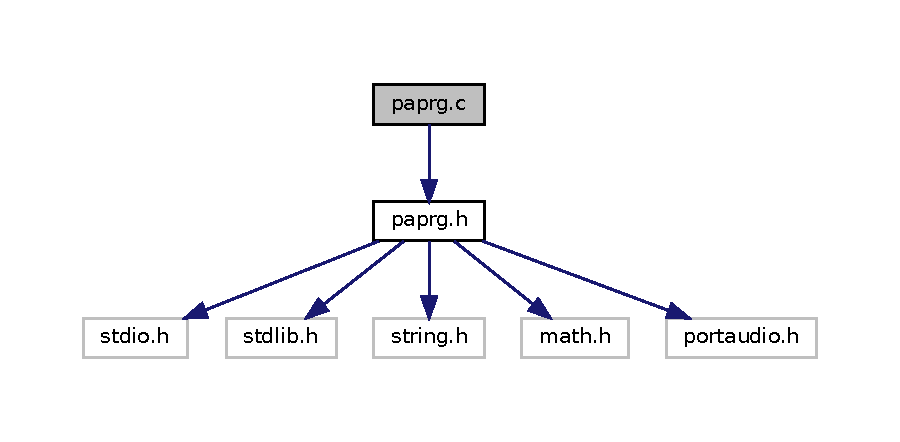
\includegraphics[width=350pt]{paprg_8c__incl}
\end{center}
\end{figure}
\subsection*{Functions}
\begin{DoxyCompactItemize}
\item 
int \hyperlink{paprg_8c_a83fd123b66ed381181358808dba1663c}{Pa\+Prg\+Play} (float frequency, unsigned int mlsec, Pa\+Stream\+Parameters $\ast$output\+Parameters)
\begin{DoxyCompactList}\small\item\em Функция, которая играет звук заданной частоты заданное время. \end{DoxyCompactList}\end{DoxyCompactItemize}


\subsection{Detailed Description}
Исходный код библиотеки 



\subsection{Function Documentation}
\mbox{\Hypertarget{paprg_8c_a83fd123b66ed381181358808dba1663c}\label{paprg_8c_a83fd123b66ed381181358808dba1663c}} 
\index{paprg.\+c@{paprg.\+c}!Pa\+Prg\+Play@{Pa\+Prg\+Play}}
\index{Pa\+Prg\+Play@{Pa\+Prg\+Play}!paprg.\+c@{paprg.\+c}}
\subsubsection{\texorpdfstring{Pa\+Prg\+Play()}{PaPrgPlay()}}
{\footnotesize\ttfamily int Pa\+Prg\+Play (\begin{DoxyParamCaption}\item[{float}]{frequency,  }\item[{unsigned int}]{mlsec,  }\item[{Pa\+Stream\+Parameters $\ast$}]{output\+Parameters }\end{DoxyParamCaption})}



Функция, которая играет звук заданной частоты заданное время. 


\begin{DoxyParams}{Parameters}
{\em frequency} & -\/ частота \\
\hline
{\em mlsec} & -\/ Время (в милисекундах). \\
\hline
{\em output\+Parameters} & -\/ Информация о устройстве вывода. \\
\hline
\end{DoxyParams}
\begin{DoxyReturn}{Returns}
\mbox{[}int\mbox{]} код ошибки 
\end{DoxyReturn}

\hypertarget{paprg_8h}{}\section{paprg.\+h File Reference}
\label{paprg_8h}\index{paprg.\+h@{paprg.\+h}}


Заголовочный файл для библиотеки  


{\ttfamily \#include $<$stdio.\+h$>$}\newline
{\ttfamily \#include $<$stdlib.\+h$>$}\newline
{\ttfamily \#include $<$string.\+h$>$}\newline
{\ttfamily \#include $<$math.\+h$>$}\newline
{\ttfamily \#include \char`\"{}portaudio.\+h\char`\"{}}\newline
Include dependency graph for paprg.\+h\+:
\nopagebreak
\begin{figure}[H]
\begin{center}
\leavevmode
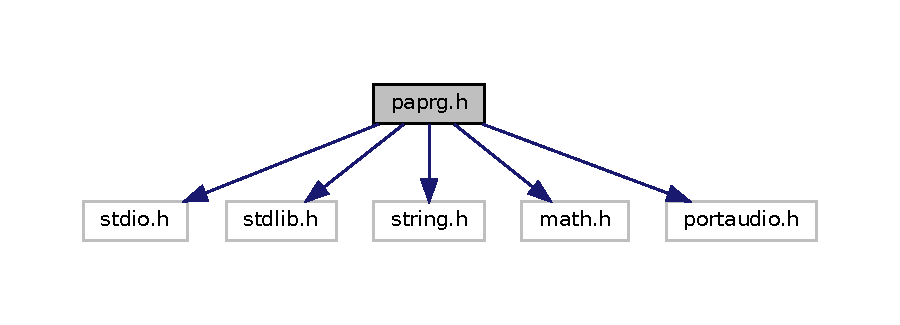
\includegraphics[width=350pt]{paprg_8h__incl}
\end{center}
\end{figure}
This graph shows which files directly or indirectly include this file\+:\nopagebreak
\begin{figure}[H]
\begin{center}
\leavevmode
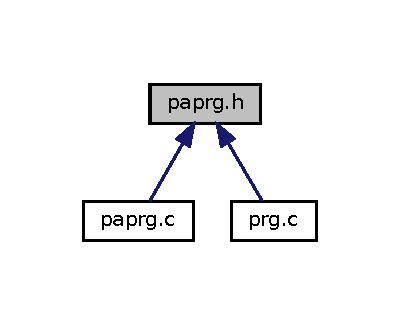
\includegraphics[width=192pt]{paprg_8h__dep__incl}
\end{center}
\end{figure}
\subsection*{Data Structures}
\begin{DoxyCompactItemize}
\item 
struct \hyperlink{struct_pa_data}{Pa\+Data}
\begin{DoxyCompactList}\small\item\em Структура для передачи данных в функцию обратного вызова. \end{DoxyCompactList}\end{DoxyCompactItemize}
\subsection*{Macros}
\begin{DoxyCompactItemize}
\item 
\mbox{\Hypertarget{paprg_8h_a4b76a0c2859cfd819a343a780070ee2b}\label{paprg_8h_a4b76a0c2859cfd819a343a780070ee2b}} 
\#define \hyperlink{paprg_8h_a4b76a0c2859cfd819a343a780070ee2b}{S\+A\+M\+P\+L\+E\+\_\+\+R\+A\+TE}~(44100)
\begin{DoxyCompactList}\small\item\em Частота дискретизации (сколько раз в секунду будет изменяться сигнал на выходное устройство) \end{DoxyCompactList}\item 
\mbox{\Hypertarget{paprg_8h_af4f62216aa14e0407faa6631e9ec4c62}\label{paprg_8h_af4f62216aa14e0407faa6631e9ec4c62}} 
\#define \hyperlink{paprg_8h_af4f62216aa14e0407faa6631e9ec4c62}{F\+R\+A\+M\+E\+S\+\_\+\+P\+E\+R\+\_\+\+B\+U\+F\+F\+ER}~(64)
\begin{DoxyCompactList}\small\item\em Буфер вывода. \end{DoxyCompactList}\item 
\mbox{\Hypertarget{paprg_8h_ae71449b1cc6e6250b91f539153a7a0d3}\label{paprg_8h_ae71449b1cc6e6250b91f539153a7a0d3}} 
\#define \hyperlink{paprg_8h_ae71449b1cc6e6250b91f539153a7a0d3}{M\+\_\+\+PI}~(3.\+14159265)
\begin{DoxyCompactList}\small\item\em Константа Pi. \end{DoxyCompactList}\end{DoxyCompactItemize}
\subsection*{Functions}
\begin{DoxyCompactItemize}
\item 
int \hyperlink{paprg_8h_a83fd123b66ed381181358808dba1663c}{Pa\+Prg\+Play} (float frequency, unsigned int mlsec, Pa\+Stream\+Parameters $\ast$output\+Parameters)
\begin{DoxyCompactList}\small\item\em Функция, которая играет звук заданной частоты заданное время. \end{DoxyCompactList}\end{DoxyCompactItemize}


\subsection{Detailed Description}
Заголовочный файл для библиотеки 



\subsection{Function Documentation}
\mbox{\Hypertarget{paprg_8h_a83fd123b66ed381181358808dba1663c}\label{paprg_8h_a83fd123b66ed381181358808dba1663c}} 
\index{paprg.\+h@{paprg.\+h}!Pa\+Prg\+Play@{Pa\+Prg\+Play}}
\index{Pa\+Prg\+Play@{Pa\+Prg\+Play}!paprg.\+h@{paprg.\+h}}
\subsubsection{\texorpdfstring{Pa\+Prg\+Play()}{PaPrgPlay()}}
{\footnotesize\ttfamily int Pa\+Prg\+Play (\begin{DoxyParamCaption}\item[{float}]{frequency,  }\item[{unsigned int}]{mlsec,  }\item[{Pa\+Stream\+Parameters $\ast$}]{output\+Parameters }\end{DoxyParamCaption})}



Функция, которая играет звук заданной частоты заданное время. 


\begin{DoxyParams}{Parameters}
{\em frequency} & -\/ частота \\
\hline
{\em mlsec} & -\/ Время (в милисекундах). \\
\hline
{\em output\+Parameters} & -\/ Информация о устройстве вывода. \\
\hline
\end{DoxyParams}
\begin{DoxyReturn}{Returns}
\mbox{[}int\mbox{]} код ошибки 
\end{DoxyReturn}

\hypertarget{prg_8c}{}\section{prg.\+c File Reference}
\label{prg_8c}\index{prg.\+c@{prg.\+c}}
{\ttfamily \#include \char`\"{}paprg.\+h\char`\"{}}\newline
Include dependency graph for prg.\+c\+:
\nopagebreak
\begin{figure}[H]
\begin{center}
\leavevmode
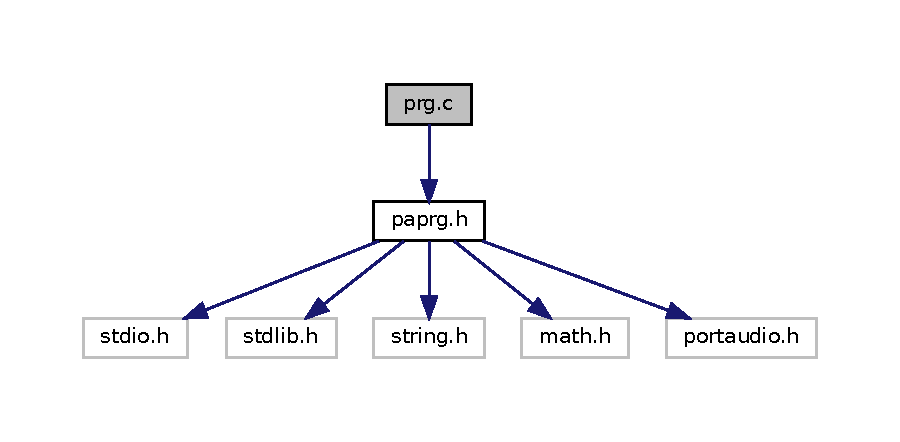
\includegraphics[width=350pt]{prg_8c__incl}
\end{center}
\end{figure}
\subsection*{Functions}
\begin{DoxyCompactItemize}
\item 
int \hyperlink{prg_8c_a840291bc02cba5474a4cb46a9b9566fe}{main} (void)
\begin{DoxyCompactList}\small\item\em Входная точка программы \end{DoxyCompactList}\end{DoxyCompactItemize}


\subsection{Function Documentation}
\mbox{\Hypertarget{prg_8c_a840291bc02cba5474a4cb46a9b9566fe}\label{prg_8c_a840291bc02cba5474a4cb46a9b9566fe}} 
\index{prg.\+c@{prg.\+c}!main@{main}}
\index{main@{main}!prg.\+c@{prg.\+c}}
\subsubsection{\texorpdfstring{main()}{main()}}
{\footnotesize\ttfamily int main (\begin{DoxyParamCaption}\item[{void}]{ }\end{DoxyParamCaption})}



Входная точка программы 

\begin{DoxyReturn}{Returns}
статус (возвратный код) программы. 
\end{DoxyReturn}
Here is the call graph for this function\+:
\nopagebreak
\begin{figure}[H]
\begin{center}
\leavevmode
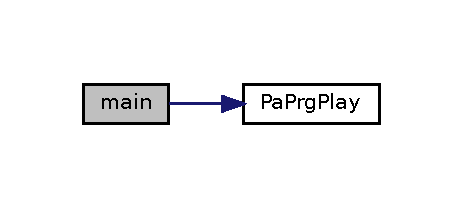
\includegraphics[width=222pt]{prg_8c_a840291bc02cba5474a4cb46a9b9566fe_cgraph}
\end{center}
\end{figure}

%--- End generated contents ---

% Index
\backmatter
\newpage
\phantomsection
\clearemptydoublepage
\addcontentsline{toc}{chapter}{Index}
\printindex

\end{document}
